%!TEX root=../../autopilot.tex
\section{Directory Structure}
\label{sec:userdir}

On setup, Autopilot creates a user directory that contains all local files that define its operation (Figure \ref{fig:userdir}). The subdirectories include:

\begin{marginfigure}[2.15cm]
\begin{minted}[frame=lines,fontsize=\small]{text}
./autopilot
├── calibration
├── data
│   ├── subject_1.h5
│   └── subject_2.h5
├── launch_autopilot.sh
├── logs
│   ├── core.terminal.log
│   └── plugins.my_plugin.log
├── pilot_db.json
├── plugins
│   └── my_plugin
│       └── my_task.py
├── prefs.json
├── protocols
│   ├── 2afc_easy.json
│   └── 2afc_hard.json
└── sounds
\end{minted}
\caption{Example user directory structure, typically in \texttt{$\sim$/autopilot}.}
\label{fig:userdir}
\end{marginfigure}

\begin{itemize}
\item \textbf{\texttt{calibration}} --- Calibration for hardware objects like audio or solenoids that, for example, map opening durations to volumes of liquids dispensed
\item \textbf{\texttt{data}} --- \hyperref[sec:datamodel]{Data} for experimental subjects
\item \textbf{\texttt{launch\_autopilot.sh}} --- Launch script that includes launching external processed like the jack audio daemon (will be removed and integrated into a more formal \hyperref[sec:agents]{agent} structure in future versions)
\item \textbf{\texttt{logs}} --- Every Autopilot object is capable of full debug logging, neatly formatted by object type and instance ID and grouped within module-level logging files. Logs are both written to disk, and output to \texttt{stderr} using the \href{https://rich.readthedocs.io/en/latest/reference/logging.html#logging}{rich logging handler} for clean and readable inspection during program operation (Figure \ref{fig:logging}). Logs can be parsed back into python objects to make it straightforward to diagnose problems or recover data in the case of an error.
\item \textbf{\texttt{pilot\_db.json}} --- A .json file that stores information about associated \hyperref[sec:agents]{Pilots}, including the contents of their prefs files, which hash/version of Autopilot they are running, and any Subjects that are associated with them.
\item \textbf{\texttt{plugins}} --- Plugins, which are any Python files that contain subclasses of Autopilot objects, that are automatically made available by Autopilot's \href{https://docs.auto-pi-lot.com/en/latest/utils/registry.html}{registry} system (eg. \mintinline{python}{autopilot.get('hardware', 'My_Hardware')} would retrieve a custom hardware object). Plugins can be documented and made available to other Autopilot users by registering them on the \href{https://wiki.auto-pi-lot.com/index.php/Autopilot_Plugins}{wiki}
\item \textbf{\texttt{prefs.json}} --- Configuration options for this particular Autopilot instance, including configurations of local hardware objects, audio output, etc. In the future this will likely be broken into multiple files for different kinds of preferences\sidenote{with care for backwards compatibility}.
\item \textbf{\texttt{protocols}} --- \hyperref[sec:tasks]{Protocols}, which consist of parameterizations of individual Tasks as well as criteria for graduating betwewen them. These are also stored in individual subject data files, and updated whenever the source protocol files change.
\item \textbf{\texttt{sounds}} --- Any sound files that are requested by the \href{https://docs.auto-pi-lot.com/en/latest/stim/sound/sounds.html\#autopilot.stim.sound.sounds.File}{File} sound class.
\end{itemize}

\begin{figure*}[hb]
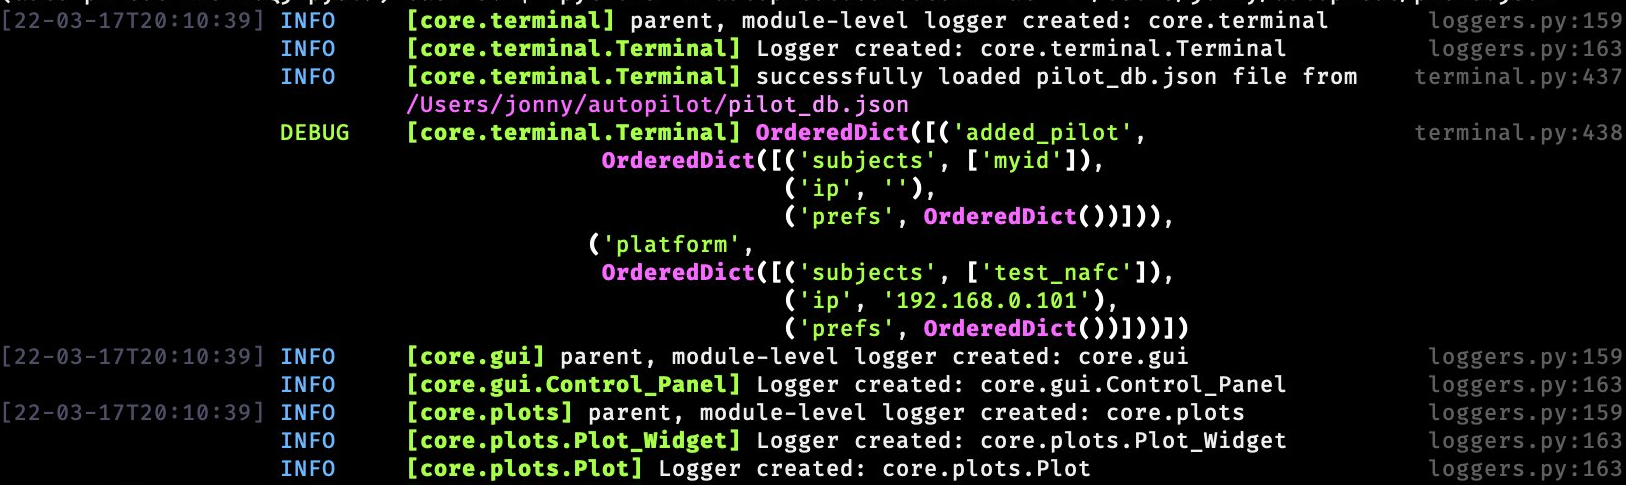
\includegraphics[width=\linewidth]{autopilot/autopilot/src/figures/logging.png}
\caption{Logs printed to \texttt{stderr} are formatted and colorized by the \href{https://rich.readthedocs.io/en/latest/reference/logging.html\#logging}{rich logging handler}. Logfiles are created by module, and log entries are identified by the individual objects instantiated from them. Logfiles are rotated and size-limited for configurable backups.}
\label{fig:logging}
\end{figure*}




